% Created 2024-06-16 Sun 21:02
% Intended LaTeX compiler: pdflatex
\documentclass[11pt]{article}
\usepackage[utf8]{inputenc}
\usepackage[T1]{fontenc}
\usepackage{graphicx}
\usepackage{longtable}
\usepackage{wrapfig}
\usepackage{rotating}
\usepackage[normalem]{ulem}
\usepackage{amsmath}
\usepackage{amssymb}
\usepackage{capt-of}
\usepackage{hyperref}
\usepackage[a4paper,left=1cm,right=1cm,top=1cm,bottom=1cm]{geometry}
\usepackage[american]{babel}
\usepackage[sc]{mathpazo}
\linespread{1.05}
\setlength\parindent{0pt}
\newcommand{\minCostPath}[2]{\mathrm{minCostPath}\left(\left\{#1\right\},#2\right)}
\newcommand{\minCostTour}[2]{\mathrm{minCostTour}\left(\left\{#1\right\},#2\right)}
\author{Marcio Woitek}
\date{}
\title{Held-Karp Algorithm}
\hypersetup{
 pdfauthor={Marcio Woitek},
 pdftitle={Held-Karp Algorithm},
 pdfkeywords={},
 pdfsubject={},
 pdfcreator={Emacs 29.3 (Org mode 9.6.24)}, 
 pdflang={English}}
\begin{document}

\maketitle
\thispagestyle{empty}
\pagestyle{empty}

All problems are related to the graph shown below. Black edges have weight 1,
and red edges have weight 2.
\begin{figure}[h]
  \centering
  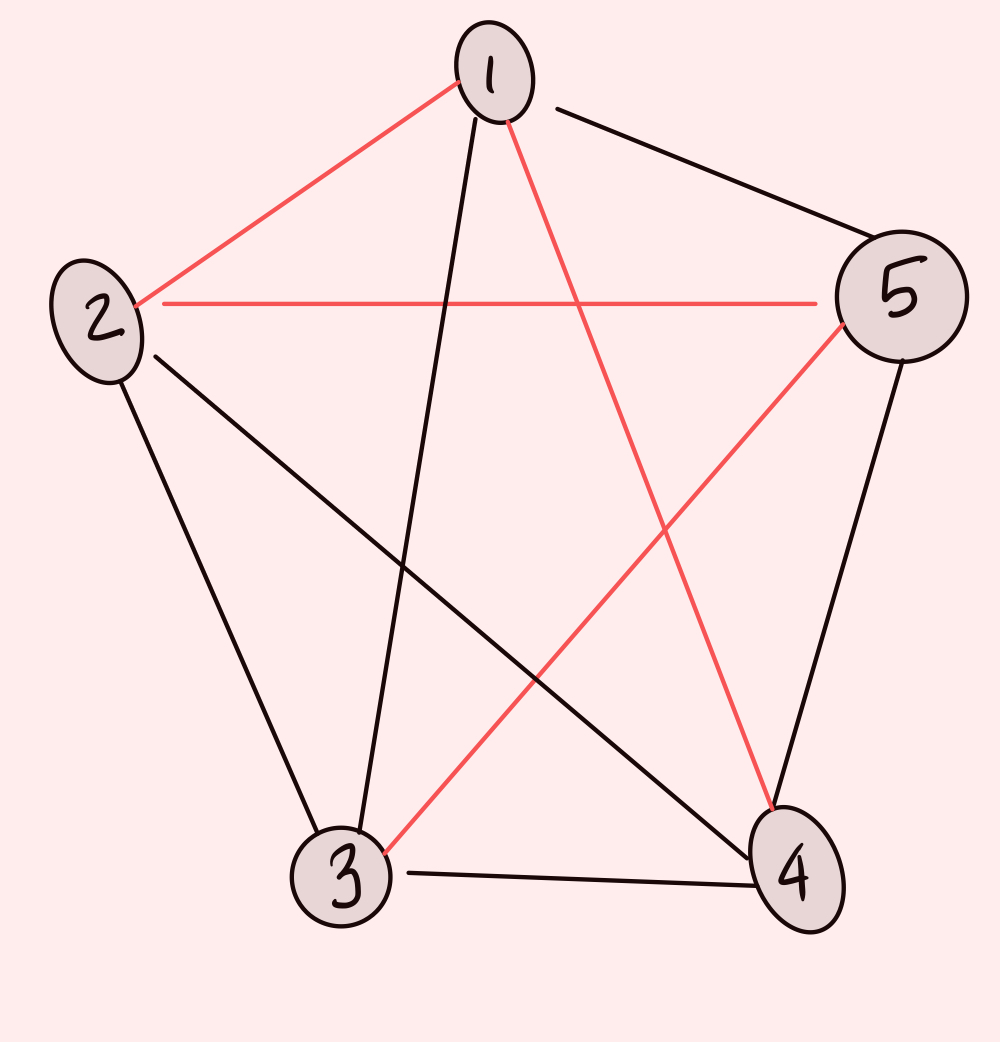
\includegraphics[scale=0.25]{held_karp_graph.jpeg}
  \caption{TSP instance}
\end{figure}

\section*{Problem 1}
\label{sec:orgae58da4}
\begin{equation}
\minCostPath{2,3}{4}=\min\left(\minCostPath{2}{3}+C_{3,4},\minCostPath{3}{2}+C_{2,4}\right)
\end{equation}

\section*{Problem 2}
\label{sec:org6bf1af5}
We begin by computing the arguments of the \(\min\) function on the RHS of the above equation:
\begin{align*}
\minCostPath{2}{3}+C_{3,4}&=C_{1,2}+C_{2,3}+C_{3,4}=2+1+1=4,\\
\minCostPath{3}{2}+C_{2,4}&=C_{1,3}+C_{3,2}+C_{2,4}=1+1+1=3.
\end{align*}
Hence:
\begin{equation}
\minCostPath{2,3}{4}=\min(4,3)=3.
\end{equation}

\section*{Problem 3}
\label{sec:org1d34b8b}
I believe the correct answer is vertex 2. After all, from the above
calculations, visiting vertex 2 before vertex 4 yields the optimal solution.
However, the answer that is accepted as correct is \textbf{vertex 3}. Perhaps I'm
wrong. But it wouldn't be the first instructor mistake I catch.

\section*{Problem 4}
\label{sec:org6bca4f2}
The correct formula for the recurrence is
\begin{equation}
\mathrm{minCostTSPTour}(C)=\min
  \begin{cases}
    \minCostTour{2,3,5}{4}+C_{4,1}\\
    \minCostTour{2,3,4}{5}+C_{5,1}\\
    \minCostTour{3,4,5}{2}+C_{2,1}\\
    \minCostTour{2,4,5}{3}+C_{3,1}
  \end{cases}
.
\end{equation}
Therefore, the missing portions are given by
\begin{align}
??_1&=C_{4,1}=2,\\
??_2&=C_{5,1}=1,\\
??_3&=2,\\
??_4&=C_{2,1}=2,\\
??_5&=\{2,4,5\},\\
??_6&=C_{3,1}=1.
\end{align}
\end{document}
